% arara: lualatex: { synctex: yes, shell: yes } 
% arara: biber 
% arara: lualatex 
% if changed(toFile("ethik.bib")) || missing(toFile("ethik.bib"))

% LTeX: language=de-DE

% % -*- coding:utf-8 -*-
\documentclass[11pt, a4paper]{scrartcl}
\nonstopmode

% Basic Packages
%\usepackage[utf8]{inputenc}
%\usepackage[T1]{fontenc}
\usepackage[ngerman]{babel}

% Geometry
\usepackage[a4paper,
            bindingoffset=0.2in,
            left=1.5in,
            right=1.5in,
            top=1in,
            bottom=1in,
            footskip=.3in]{geometry}
            
% Textstuff
\usepackage{csquotes}
\usepackage{url}
\usepackage{hyperref}
\usepackage{lmodern}            % Provides the Latin Modern Font which offers more glyphs than the default Computer Modern
\usepackage[nameinlink]{cleveref}
\crefname{figure}{Abbildung}{Abbildung}
\crefname{subfigure}{Abbildung}{Abbildung}
\crefname{table}{Tabelle}{Tabelle}
\crefname{listing}{Quelltext}{Quelltext}
\crefname{chapter}{Kapitel}{Kapitel}
\crefname{section}{Abschnitt}{Abschnitt}
\crefname{subsection}{Abschnitt}{Abschnitt}
\crefname{subsubsection}{Abschnitt}{Abschnitt}
\crefname{beispiel}{Beispiel}{Beispiel}
\crefname{lemma}{Lemma}{Lemma}

% Set Paragraph Skip
\setlength{\parskip}{0.5\baselineskip}%
\setlength{\parindent}{0pt}%

% gfx
\usepackage{pgfpages}
\usepackage{svg}
\usepackage{graphicx}
\usepackage{xcolor}
\usepackage{color}
\usepackage{wrapfig}

% Tikz
\usepackage{tikz}
\usetikzlibrary{positioning,calc}

% Bibliography
\usepackage{biblatex}
\addbibresource{ethik.bib}




\title{Faites Vos Jeux}
\subtitle{So viele Daten sind das ja nicht... oder?}
\author{Etienne Palanga}
\date{\today}


\begin{document}

\maketitle

\tableofcontents

\newpage
\begin{frame}{Datenschutz}
  \centering 
  
  \note[item]{Überall werden Daten erhoben}
  \note[item]{
    Manchmal eindeutig 
    \begin{itemize}
      \item Eingabe von Daten bei Kontoerstellung
    \end{itemize}
  }
  \note[item]{
    Aber viel öfter ohne wirkliches Wissen
    \begin{itemize}
      \item Tracker auf Websites
      \item Nutzung anderer Dienste
    \end{itemize}
  }
  \note[item]{
    Deswegen Datenschutz wichtig
  }

  
\includegraphics[width=0.45\textwidth]{images/computer_data_tobu} 
\end{frame}

\begin{frame}{Datenschutz}

  \note<1->[item]{Definition aus Paper von Lee et al. (meine Zusammenfassung u. Übersetzung)}
  \note<2->[item]{Schutz vor unauthorisiertem Zugriff}
  \note<3->[item]{Sicherung, dass die Daten angemessen genutzt werden}
  \note<4->[item]{Korrektheit und Vollständigkeit gesammelter Daten über Personen}
  \note<5->[item]{Verfügbarkeit der Daten für das Subjekt und die Sicherung der Rechte des Subjekts an seinen Daten}
  \note<6->[item]{Sicherung der Rechte des Subjekts die Daten einzusehen, aktualisieren oder korrigieren}

  Nach Lee et al.\cite{lee_ethical_2016}:

  \begin{block}{Datenschutz}
    \begin{itemize}
      \item<2->{Schutz vor unauthorisiertem Zugriff}
      \item<3->{Sicherung, dass die Daten angemessen genutzt werden}
      \item<4->{Korrektheit und Vollständigkeit gesammelter Daten über Personen}
      \item<5->{Verfügbarkeit der Daten für das Subjekt und das Besitzrecht des Subjekts an seinen Daten}
      \item<6->{Sicherung der Rechte des Subjekts die Daten einzusehen, aktualisieren oder korrigieren}
    \end{itemize} 
  \end{block}
\end{frame}

\begin{frame}{Datenschutz}
  \centering

  \note<1->[item]{Selbes Paper}
  \note<1->[item]{Gesetz und Ethik sind verbunden}
  \note<2->[item]{Gesetz gibt Ethik Durchsetzungsvermögen \begin{itemize}
      \item Bsp. Ethischer Schluss: Stehlen ist falsch
      \item Aber ohne Gesetz: keine Durchsetzung
    \end{itemize}
  }
  \note<3->[item]{Ethik gibt Gesetz Kontext \begin{itemize}
      \item Bsp. Arbeit in Niedriglohnländer auszulagern ist legal, aber ist es ethisch?
    \end{itemize}
  }
  \note<3->[item]{Ethische Ideen über Datenschutz werden im Gesetz umgesetzt.}
  \note<3->[item]{Sehen das später etwas mehr}

  \begin{tikzpicture}
    \node (law) {
\includegraphics[width=0.25\textwidth]{images/book_law}};
    \node[below = 0cm of law] (law-name) {Gesetz};
    \node[right = 4cm of law] (ethics) {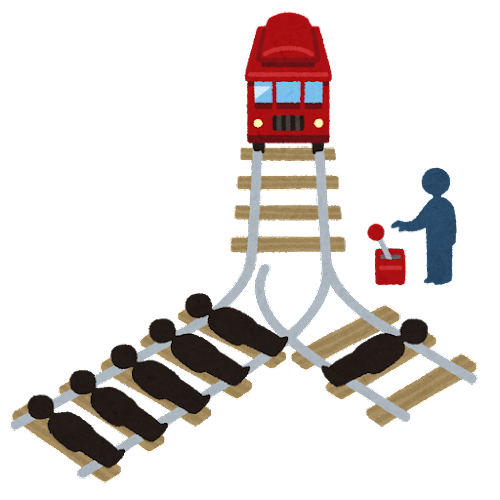
\includegraphics[width=0.25\textwidth]{images/trolley_problem}};
    \node[below = 0cm of ethics] (ethics-name) {Ethik};

    \draw<2->[-stealth] (law) to[out = 20, in = 160, edge node={node[above] {Kann durchsetzen}}] (ethics);
    \draw<3->[-stealth] (ethics) to[out = 200, in = 340, edge node={node[below] {Gibt Kontext}}] (law);
  \end{tikzpicture}

\end{frame}


\newpage
\section{Grundlagen}

Zunächst wollen wir uns mit dem Zusammenhang von Gesetz und Ethik, sowie mit Datenschutz auseinandersetzen.
Ersteres ist wichtig für die spätere Evaluation des Fallbeispiels,
während Letzteres das Fundament für die Diskussion der Hauptthematik des Fallbeispiels bildet.

\subsection{Gesetz und Ethik}
\label{sec:02:lawethics}

\begin{wrapfigure}{r}{0.4\textwidth}
    \centering
    \begin{tikzpicture}[text node/.style={font=\sffamily\small}]
        \node (law) {
\includegraphics[width=0.25\textwidth]{images/book_law}};
        \node[text node, below = 0cm of law] (law-name) {Gesetz};
        \node[below = 3cm of law-name] (ethics) {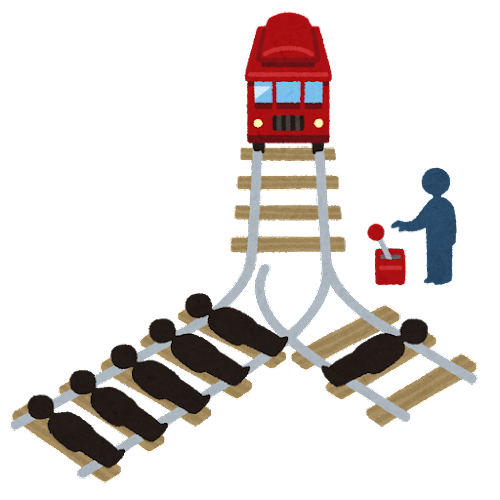
\includegraphics[width=0.25\textwidth]{images/trolley_problem}};
        \node[text node, below = 0cm of ethics] (ethics-name) {Ethik};

        \draw[-stealth, blue] (law) to[out = 300, in = 60, edge node={node[above left, text node] {\small Kann durchsetzen}}] (ethics);
        \draw[-stealth, red] (ethics) to[out = 120, in = 240, edge node={node[below right, text node] {\small Gibt Kontext}}] (law);
    \end{tikzpicture}
    \caption{Wechselwirkung von Gesetz und Ethik.}
    \label{fig:02:lawethics}
\end{wrapfigure}

So wie Privatsphäre, Sicherheit und Vertrauen verwandt sind, so sind es auch Ethik und das Gesetz.
Auf der einen Seite bietet das Gesetz einem ethischen Prinzip die Möglichkeit, 
das Prinzip tatsächlich in der Gesellschaft durchzusetzen.\cite{lee_ethical_2016}

Beispielsweise kann man aufgrund eines individuellen ethischen Verständnisses zu dem Schluss kommen, dass stehlen falsch ist.
Es ist natürlich auch so, dass die meisten Menschen dieses Verständnis im Allgemeinen teilen.
Allerdings ist das allein nicht genug, damit dieses Verständnis in der Gesellschaft auch durchgesetzt werden kann.
Denn einerseits kann es Menschen geben, die zwar dieses gleiche Verständnis besitzen, dies aber brechen.
Andererseits kann es auch sein, dass Menschen dieses Verständnis nicht teilen und aus diesem Grund stehlen.
Das Gesetz kann nun durch den Staat dieses Verständnis umsetzen, indem die,
die dieses Gesetz -- und damit das ethische Prinzip -- brechen, strafrechtlich verfolgt werden können.

Auf der anderen Seite bietet Ethik Kontext für bestehende Gesetze.
Ein Beispiel hierfür ist etwa das Auslagern von Arbeitsplätzen in ein Niedriglohnland.
Dies ist zwar hierzulande legal, allerdings lässt es sich streiten, ob dies ethisch korrekt ist.

Zudem existieren unbestimmte Rechtsbegriffe, wie hierzulande beispielsweise \enquote{Treu und Glauben} (zum Beispiel §~242 BGB).
Dieser sagt aus, dass man sich um dem jeweiligen Gesetz zu entsprechen \enquote{anständig und redlich verhalten} habe.\cite{alexy_treu_2019}
Wenn also festgestellt werden soll, ob eine Person entsprechend \enquote{Treu und Glauben} gehandelt hat,
können durchaus auch ethische Überzeugungen mit einfließen.

Diese Wechselwirkung ist in \cref{fig:02:lawethics} visualisiert.

Wie bereits in diesem Beispiel angedeutet, können Gesetze auch oft aus ethischen Überzeugungen entstehen.
Daher kann es bei der Evaluation ethischer Vertretbarkeit einer Handlung auch von Nutzen sein,
die gesetzliche Lage zu betrachten, sollten die zugrundeliegenden ethischen Überzeugungen erkennbar sein.

\subsection{Privatsphäre, Sicherheit und Vertrauen}

\begin{wrapfigure}{l}{0.6\textwidth}
    \centering
    \begin{tikzpicture}[text node/.style={font=\sffamily\small}]
        \node at (30:3cm) (privacy) {
\includegraphics[width=0.15\textwidth]{images/secret}};
        \node[text node, below = 0cm of privacy] (privacy-name) {Privatsphäre};
        \node at (150:3cm) (security) {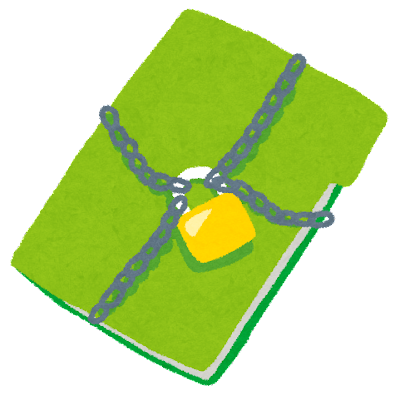
\includegraphics[width=0.15\textwidth]{images/lock_file}};
        \node[text node, below = 0cm of security] (security-name) {Sicherheit};
        \node at (270:3cm) (trust) {
\includegraphics[width=0.15\textwidth]{images/handshake}};
        \node[text node, below = 0cm of trust] (trust-name) {Vertrauen};
        
        \draw[stealth-stealth] (privacy) edge[bend right] node [text node, above] {Bedingen einander} (security);
        \draw[-stealth] (security-name) edge[bend right] node [text node, left] {\small Benötigt} (trust);
        \draw[stealth-] (trust) edge[bend right] node [text node, right] {Benötigt} (privacy-name);
    \end{tikzpicture}
    \caption{Wechselwirkungen von Sicherheit, Privatsphäre und Vertrauen.}
    \label{fig:02:secprivtru}
\end{wrapfigure}

Ebenfalls beschreiben Lee et al., dass die Gewährleistung von Privatsphäre und Sicherheit
eng mit dem Vertrauen in Dritte auch eine Wechselwirkung haben.\cite{lee_ethical_2016}
Soll die Privatsphäre einer Person geschützt, oder die Sicherheit einer Person garantiert werden, insbesondere durch Dritte,   
so muss Vertrauen in diese Dritten herrschen.

In beiden Fällen muss den Dritten Zugang zu dem privaten Bereich der Person gegeben werden.
Soll im Fall von Privatsphäre beispielsweise eine andere Person das eigene Tagebuch verwahren,
so muss das Vertrauen in diese andere Person herrschen, dass diese nicht selbst unerlaubt in dem Tagebuch liest.
Im Allgemeinen muss man Anderen vertrauen können, sollte man diesen Zugriff auf einen privaten Bereich geben. 

Im Falle Sicherheit muss zum Beispiel ein Bodyguard nah bei der zu beschützenden Person bleiben.
Dabei muss natürlich das Vertrauen herrschen, dass der Bodyguard selbst keine schlechten Absichten hat.
Allgemeiner, muss einem \enquote{Anbieter} von Sicherheit vertraut werden, dass dieser seine Arbeit gut und gewissenhaft tut.

Diese Zusammenhänge sind in \cref{fig:02:secprivtru} visualisiert.

Diese Aspekte finden sich im Datenschutz ebenfalls wieder.

\subsection{Datenschutz}

Datenschutz befasst sich mit dem Umgang mit den privaten Daten eines Subjekts.
Dazu zählt etwa wie auf diese zugegriffen werden darf, wie sie gesammelt werden dürfen oder von einer dritten Partei genutzt werden dürfen.
Besondere Wichtigkeit haben hier die Rechte, die das Subjekt selbst an ihren eigenen Daten hat.
Die Hauptaspekte lassen sich folgendermaßen zusammenfassen:\cite{lee_ethical_2016}  

\begin{center}
\parbox{0.9\textwidth}{
    Eine Instanz, die Daten Anderer verwaltet und Datenschutz betreibt, muss folgendes gewährleisten: 
    \begin{itemize}
        \item Schutz vor unauthorisiertem Zugriff
        \item Sicherstellen angemessener Benutzung der Daten
        \item Richtigkeit und Vollständigkeit gesammelter Daten über Personen oder Firmen
        \item Verfügbarkeit der Daten für das Subjekt und das Recht des Subjekts die Daten zu besitzen
        \item Das Recht des Subjekts, die Daten zu inspizieren, zu aktualisieren oder zu korrigieren
    \end{itemize}
}
\end{center}

Solange die Daten allein in der Hand ihres Eigentümers oder Eigentümerin sind, ist kein Datenschutz vonnöten,
da es hier unstrittig ist, ob auf die Daten zugegriffen werden darf oder ob sie verwendet werden dürfen.
Wir befassen uns also damit, was gelten soll, wenn die Daten in die Hände Anderer übergeben werden.

Wie wir bereits gesehen haben, hängen Privatsphäre, Sicherheit und Vertrauen zusammen. 
Dies ist auch bei Datenschutz nicht anders. Denn all diese drei Aspekte sind für Datenschutz nötig.
Durch den Schutz der privaten Daten des Subjekts wird dessen \emph{Privatsphäre} gewahrt.
Darüber hinaus muss die Daten schützende Instanz, die Daten in Hinblick auf die oben genannten Aspekte \emph{absichern}.
Die Instanz, die dies durchführt, benötigt das \emph{Vertrauen} dies gewissenhaft durchzuführen.

\subsubsection{Konsequenzen mangelnden Datenschutzes}

Natürlich ist Datenschutz aus dem Grund nötig, dass das Nicht-Schützen von Daten negative Konsequenzen mit sich zieht.
Dementsprechend muss sich Datenschutz auch mit diesen befassen, damit solche negativen Konsequenzen nach Möglichkeit vermieden oder zumindest vermindert werden können.
Nach Lee et al. lassen sich diese Konsequenzen in sogenannte \emph{Soft Costs} und \emph{Hard Costs} aufteilen. \cite{lee_ethical_2016}

Dabei handelt es sich bei Hard Costs um materielle Konsequenzen, wie finanzielle oder durch strafrechtliche Verfolgung entstehende Kosten.

Soft Costs sind dabei andere Konsequenzen, wie zum Beispiel der Verlust des Vertrauens der Kunden oder der Verlust eines guten Rufs.

\paragraph*{Facebook Datenleck 2021}

Ein Beispiel für solche negativen Konsequenzen ist ein Datenleck bei Facebook\footnote{\url{https://www.facebook.com/}}, 
der im Jahr 2021 entdeckt wurde.\cite{holmes_533_2021}
Hier wurden in 2021 die Daten von über \emph{533 Millionen} Nutzern und Nutzerinnen veröffentlicht.
Diese Daten beinhalten die Facebook IDs, Namen, Wohnorte, Geburtsdaten und weitere private Daten.
Nach Aussage von Facebook konnten die Daten aufgrund einer Sicherheitslücke in 2019 von Facebook erhoben werden.\cite{clark_facts_2021}

Die Veröffentlichung solcher Datensätze kann Identitätsdiebstahl vereinfachen.
Böswillige Parteien können mithilfe dieser Daten andere Personen imitieren um so potentiell an weitere persönliche Daten zu gelangen.

Zu diesem Vorfall sagte Alon Gal, der technische Direktor des Cyberkriminalität-Intelligenz-Unternehmens Hudson Rock\footnote{\url{https://www.hudsonrock.com/}} (übersetzt):
\blockquote[\cite{holmes_533_2021}]{
    Individuen, die sich bei einem reputablen Unternehmen wie Facebook registrieren, vertrauen ihnen mit ihren Daten
    und Facebook sollte mit den Daten mit höchstem Respekt umgehen. [\dots] 
    Dass die persönlichen Daten von Nutzern geleakt wurden, ist ein riesiger Vertrauensbruch und sollte auch so behandelt werden.
}

Auch aus diesem Zitat sehen wir, dass die Themen Vertrauen, Privatsphäre und Sicherheit sehr große Bedeutung für Datenschutz haben. 

Obwohl die genaue Wahrnehmung von Privatsphäre sich etwas von Kultur zu Kultur unterscheiden mag,
gibt es einen groben Konsens, dass Privatsphäre ein wichtiges, sozial vorteilhaftes Gut ist.\cite{lee_ethical_2016}

Zum Thema Datenschutz betrachten wir nun das Fallbeispiel \enquote{Faites Vos Jeux}\cite{kees_faites_2017} aus dem Informatik Spektrum 2017.

\section{Faites Vos Jeux}

Zum Thema Datenschutz betrachten wir nun das Fallbeispiel \enquote{Faites Vos Jeux} \cite{kees_faites_2017} aus dem Informatik Spektrum 2017.

\subsection{AC-Games in Not}

\begin{wrapfigure}{r}{0.5\textwidth}
    
  \begin{tikzpicture}[text node/.style={font=\sffamily\small}]

    \node (walter) {
\includegraphics[width=0.15\textwidth]{images/walter.png}};
    \node[text node, below=0mm of walter] (walter-name) {Walter};
    
    \node[below=2cm of walter] (acgames) {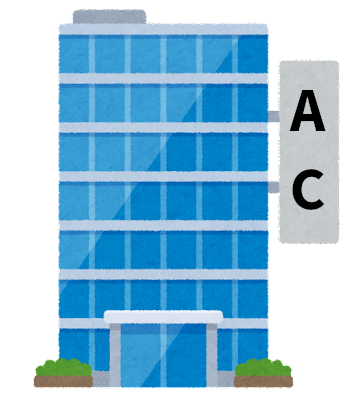
\includegraphics[width=0.15\textwidth]{images/ac_games.png}};
    \node[text node, below=0cm of acgames] (acgames-name) {AC-Games};
    
    \node[left=2.1cm of acgames] (nutzer) {
\includegraphics[width=0.15\textwidth]{images/game_friends.png}};
    \node[text node, below=0cm of nutzer] (nutzer-name) {Nutzer:innen};
    
    
    \draw[-stealth] (walter-name) -- node[text node, left] (ceo) {CEO}  (acgames);
    
    % Finanzkrise 2
    
    \draw[-stealth, red] (nutzer) -- node[text node, below] (geld) {Geld} (acgames);
    
    \node[above=1cm of geld] (finanzkrise) {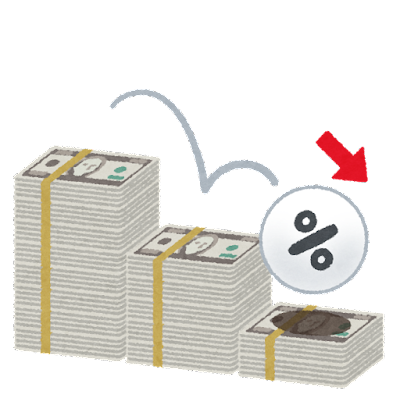
\includegraphics[width=0.10\textwidth]{images/money_down.png}};
    \node[text node, below=0cm of finanzkrise] (finanzkrise-name) {Finanzkrise};
    \draw[dotted, red] (finanzkrise-name) -- (geld);
    
    % App Stores machen obsolet 3
    
    \node[below=0.3cm of geld] (apps) {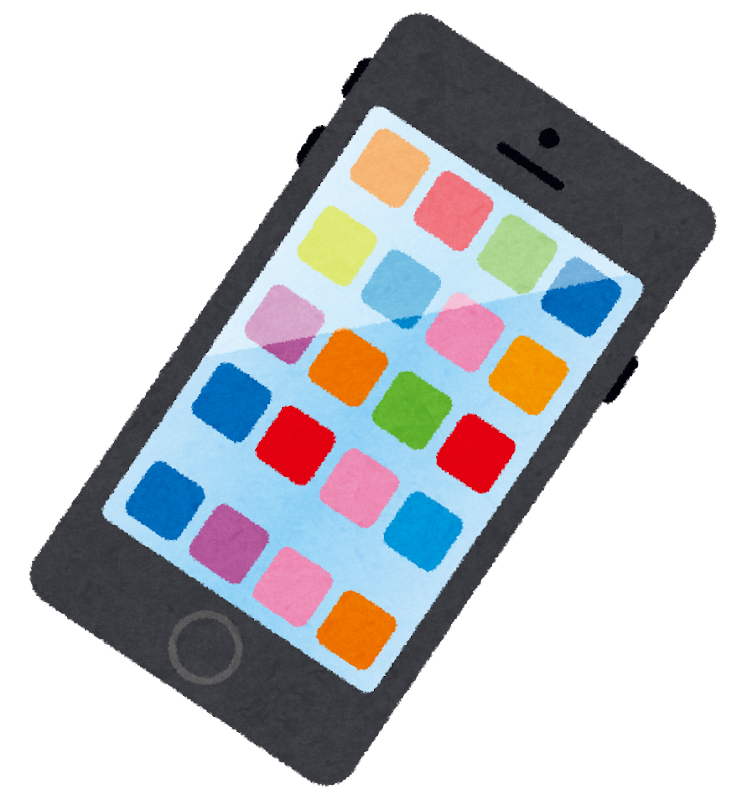
\includegraphics[width=0.08\textwidth]{images/smartphone.png}};
    \node[text node, below=0cm of apps] (apps-name) {App-Stores};
    \draw[dotted, red] (apps) -- (geld);
    
  \end{tikzpicture} 
  \caption{Die Situation von AC-Games.}
  \label{fig:03:acgamessituation}
\end{wrapfigure}

Walter ist seit nun fast 2 Jahrzehnten Geschäftsführer einer kleinen Spielfirma namens AC-Games, 
die ein kostenloses Spieleportal für Online-Spiele betreibt. (siehe \cref{fig:03:acgamessituation})
Lange Zeit lief das Geschäft gut, die Firma hatte einen gesunden Stamm von Nutzern und Nutzerinnen.
Die Einnahmen setzten sich aus Käufen virtueller Gegenstände, sowie Werbeeinnahmen zusammen.
Allein durch die 100 meist-zahlenden Nutzern und Nutzerinnen konnte AC-Games seine Kosten decken.

Doch dann begann vor etwa 10 Jahren die Wirtschaftskrise. 
Seitdem ging es mit AC-Games langsam bergab.
Dies war allerdings nicht allein der Wirtschaftskrise geschuldet.
Weitere Entwicklungen über die letzten 10 Jahre wirkten sich ebenfalls negativ auf AC-Games aus.

Beispielsweise wurden durch die Ausbreitung von Smartphones auch die damit einhergehenden App-Stores zum Problem für AC-Games.
Vor allem für Gelegenheitsspieler eignen sich Spiele aus solchen App-Stores 
und löst damit einen wichtigen Teil von Spieleportalen ab.
Darüber hinaus führte die Popularität von App-Stores dazu,
dass Spielentwickler weniger dazu geneigt waren, Spiele für Spieleportale zu entwickeln, im Vergleich zu App-Stores.
Darüber hinaus sanken auch sowohl die Werbeeinnahmen, sowie die Zahl der Käufe virtueller Gegenstände
und seit etwa 2-3 Jahren hat AC-Games Schwierigkeiten die eigenen Mitarbeiter und Mitarbeiterinnen zu bezahlen.

\subsection{Das Angebot}

Zu diesem Zeitpunkt bekommt Walter ein Angebot:
Ein Datenhändler namens \emph{Data Broker GmbH} möchte die Firma übernehmen und bietet eine sehr große Geldsumme.
Die hohe Geldsumme verwunderte die Mitglieder von AC-Games,
doch nach einer Diskussion entschließt sich Walter, die Firma an Data Broker zu übergeben.
Der Hauptgrund für diese Entscheidung, ist Walters Ansicht, dass AC-Games nur für Transaktionen nötige Daten speichert.
Es sei unproblematisch, diese Daten an Data Broker zu übergeben.

Doch tatsächlich speicherte AC-Games mehr Daten als von Walter angenommen.
Hierzu müssen wir an den Anfang von AC-Games zurückgehen.
Zu dieser Zeit war es Walter und seinen Mitgründern nicht sehr wichtig, auf Datenschutz zu achten.

In einem alten Blogpost stellt Walter seine Gedanken über eine sogenannte \emph{ultimative Slot-Machine} dar.
Diese soll ein Glücksspiel sein, das sich den Spielern und Spielerinnen anpasst.
Dazu müssten natürlich Verhaltensdaten gesammelt werden.
Darüber hinaus wurden weiter Überlegungen angestellt, wozu solche Daten noch dienen könnten.
Dies wurde aber ausschließlich intern besprochen.
Beispielsweise könne man Spielern künstlichem Stress aussetzen, um ihr Entscheidungsverhalten zu ihren Ungunsten zu beeinflussen.
Diese Ideen wurden allerdings wieder verworfen, inklusive der ultimativen Slot-Machine.

Allerdings wurden die angesprochenen Verhaltensdaten tatsächlich von AC-Games gesammelt und auch bis heute gespeichert.
Eine Mitarbeiterin namens Kathleen war die einzige, die einen Überblick darüber hatte, welche Daten nun tatsächlich gesammelt und gespeichert wurden.
Doch konnte sie mangels Ressourcen die Systeme nicht umprogrammieren, um die Datensammlung zu beenden.

Es wurde auch in einem Datenschutzaudit angemerkt, dass die Menge der gesammelten Daten eigenartig sei.
Allerdings wurde diesbezüglich nichts unternommen, da dies rechtlich legitim schien
und die Nutzer und Nutzerinnen in AGB eingewilligt haben, die diese Datensammlung erlauben.

Tatsächlich hat dieser Datenschutzaudit Data Broker erst auf AC-Games aufmerksam gemacht, da dieser öffentlich zugänglich war.
Im Idealfall für Data Broker müssten auch nicht die AGB geändert werden, 
sodass die Übernahme sogar ohne das Mitwissen der Nutzer und Nutzerinnen geschehen kann. 

\subsection{Der Wert der Daten}

\begin{wraptable}{l}{0.5\textwidth}
   \begin{tabular}{c|lll} 
        \textbf{Typ} & \textbf{Nutzer} \\\hline
        Stress & Bob L. & Lina M. & \dots \\\hline
        Neugier & Katie A. & Chris O. & \dots \\ \vdots & \dots & & 
    \end{tabular} 
    \caption{Hanks Kategorisierung der Nutzer und Nutzerinnen.}
    \label{tab:03:categories}
\end{wraptable}

Hank ist ein neuer Mitarbeiter bei AC-Games und der Datenbankadmin.
Auch er weiß von der Übernahme durch Data Broker und ist über die hohe Geldsumme verwundert.
Er schließt dadurch, dass die Daten von AC-Games nicht wertlos sind.
Da er von Walters alten Blog—Posts weiß und er nicht die Absicht hat, lange bei AC-Games zu bleiben,
ist er bereit etwas zu experimentieren.

Er stellt Berechnungen auf den Daten an und kategorisiert so die Nutzer und Nutzerinnen in verschiedene Gruppen. (siehe \cref{tab:03:categories})
Mithilfe dieser Daten fügt er dem In-Game Shop ein neues Element hinzu.
Er fügt einen Zähler hinzu, der die verbleibende Anzahl jedes Produkts darstellen soll.
Die angezeigte Zahl ist aber unecht.

Er passt die genaue Darstellung dieses Zählers auf die Nutzer und Nutzerinnen der Kategorien an,
die er mithilfe der Berechnungen erstellt hat.
So wird für \enquote{Stress-Typen} der Zähler zu Anfang auf eine zweistellige Zahl gesetzt und diese Zahl langsam dekrementiert.
Bei \enquote{Neugier-Typen} hingegen wird stattdessen ein \enquote{Vorrat prüfen}-Knopf angezeigt.
Wird dieser geklickt, wird ein Fenster mit dem Text \enquote{Nur noch ein Exemplar verfügbar!} angezeigt.

Am nächsten Tag prüft Hank die Verkaufszahlen und bemerkt, dass sich diese signifikant erhöht haben.
Er fragt sich, was noch mit diesen Daten angestellt werden könnte und überlegt, was er in dieser Situation tun sollte.
Er hat zwar Anweisungen bekommen, nicht tief in die Datenbank einzugreifen,
doch spielt er mit dem Gedanken, entgegen dieser Anweisungen zu handeln.
Auch entscheidet er sich dagegen, Walter von den Daten zu erzählen.

Schließlich entscheidet er sich, entgegen seinen Anweisungen, die Datenbank zu modifizieren.
Er pseudonymisiert die Nutzer-IDs und speichert eine Zuordnungstabelle auf seinem USB-Stick. 
\section{Ethische Grundlagen}

Im Folgenden möchte ich einige ethische Fragestellungen anhand von drei Grundlagen behandeln.
Zunächst behandlen wir die Datenschutz Grundverordnung (DSGVO) und die International Data Privacy Principles \cite{zankl_international_2014} von Wolfgang Zankl.
Zuletzt betrachten wir noch den Utilitarismus.

\subsection{Datenschutz Grundverordnung}

Die \emph{Datenschutz Grundverordnung} (DSGVO) ist eine EU-Verordnung, die den Umgang mit Personendaten regelt.
Wie bereits in \cref{sec:02:lawethics} besprochen, ist es auch nicht nutzlos, die Gesetzeslage zu betrachten.
Dies gilt insbesondere, wenn die ethischen Hintergründe bekannt sind, aus denen die Gesetze entstanden sind.

In der DSGVO finden wir in Artikel 1:
\blockquote{
    (1) Diese Verordnung enthält Vorschriften zum Schutz natürlicher Personen bei der Verarbeitung personenbezogener Daten und zum freien Verkehr solcher Daten.

    (2) Diese Verordnung schützt die Grundrechte und Grundfreiheiten natürlicher Personen und insbesondere deren Recht auf Schutz personenbezogener Daten.

    (3) Der freie Verkehr personenbezogener Daten in der Union darf aus Gründen des Schutzes natürlicher Personen bei der Verarbeitung personenbezogener Daten weder eingeschränkt noch verboten werden.
}

Wir sehen hier, dass als Grundlage für die DSGVO gilt, dass jede Person ein \enquote{Recht auf Schutz personenbezogener Daten} besitzt (Nr. 2), 
natürliche Personen, in Hinblick auf die Verarbeitung und Verkehr der persönlichen Daten, schutzbedürftig ist (Nr. 3) und diese Rechte zu schützen sind (Nr. 1).

Wir betrachten Auszüge aus der DSGVO, die für dieses Fallbeispiel relevant sind:

Sollen die Daten einer Person verarbeitet werden, so muss die Art und der Umfang der Verarbeitung für diese Person nachvollziehbar und transparent beschrieben werden (Art. 5 Nr. 1a) DSGVO).

Darüber hinaus muss ein legitimer Zweck (oder mehrere), dem die Sammlung und Verarbeitung der Daten gewidmet ist, eindeutig und verständlich festgehalten werden. Eine diesem Zweck nicht entsprechende Verarbeitung der Daten ist unzulässig (Art. 5 Nr. 1b) DSGVO). Natürlich muss die Person der Verarbeitung der Daten zu diesem Zweck zustimmen (Art. 6 Nr. 1a) DSGVO).
Damit geht einher, dass die gesammelten Daten auf das Notwendige beschränkt sind.
Demnach dürfen keine Daten gesammelt werden, die für den festgelegten Zweck nicht vonnöten sind (Art. 5 Nr. 1c) DSGVO).

Auch wenn Daten bereits erhoben sind, sind sie nun nicht Eigentum derjenigen Instanz, die diese erhoben hat. Denn sollten bereits erhobene Daten nicht mehr zur Erfüllung des Zwecks notwendig sein, müssen diese im Allgemeinen gelöscht werden (Art. 5 Nr. 1e) DSGVO).
Dabei muss sichergestellt werden, dass die Daten vor unberechtigtem Zugriff und unzulässiger Verarbeitung geschützt sind (Art. 5 Nr. 1f) DSGVO).

Die Instanz, die die Daten erhebt und verarbeitet ist dafür verantwortlich, die angesprochenen Regelungen einzuhalten (Art. 5 Nr. 2 DSGVO).


\subsection{International Data Privacy Principles}

Die \emph{International Data Privacy Principles} \cite{zankl_international_2014} (IDPP) sind 13 ethische Prinzipien für den Umgang mit Daten.
Diese wurden von Wolfgang Zankl vom Institut für Zivilrecht in Wien erarbeitet und in Harvard University\footnote{\url{https://www.harvard.edu/}}, sowie in der Computer Ethics Society Hong Kong\footnote{\url{http://www.iethicssoc.org/}} diskutiert.
Sie beziehen die Datenschutzstandards verschiedener Länder in Amerika, Asien, Europa, sowie internationale Datenschutzstandards mit ein.

Auch hier betrachten wir nur die Prinzipien, die zu diesem Fallbeispiel passen.

\paragraph*{Prinzip 1}

Eine Firma, die persönliche Daten nutzt, soll die jeweiligen nationalen Regelungen einhalten, die Datenschutz als Gegenstand haben.

\paragraph*{Prinzip 2}

Eine Firma, die persönliche Daten nutzt, soll durch Einhalten aktueller Sicherheitsstandards, unbefugten Zugriff und Verarbeitung, sowie Löschung und Verlust zu verhindern.

\paragraph*{Prinzip 3}

Eine Firma, die persönliche Daten nutzt, soll eine für Kunden einfach verständliche Datenschutzrichtlinie aufstellen und den Kunden erlauben, die verantwortliche Person persönlich zu kontaktieren.
Darüber hinaus muss die Richtlinie beschreiben, welche Daten zu welchem Zweck erhoben werden [und] wie die Daten genutzt werden [\dots].

\paragraph*{Prinzip 5}

Eine Firma, die persönliche Daten nutzt, soll Daten nicht an unauthorisierte Dritte weiter geben, es sei denn [\dots] der Kunde hat zugestimmt.

\paragraph*{Prinzip 6}

Eine Firma, die persönliche Daten nutzt, soll nur nötige Daten sammeln.

\paragraph*{Prinzip 7}

Eine Firma, die persönliche Daten nutzt, soll die gesammelten Daten auf faire Art und Weise benutzen [\dots] und nur zum Zweck, der für die Tätigkeit der Firma nötig ist.

\paragraph*{Prinzip 8}

Eine Firma, die persönliche Daten nutzt, soll keine Daten an Instanzen weiter geben, die internationale Datenschutzstandards nicht einhalten.

\paragraph*{Prinzip 10}

Eine Firma, die persönliche Daten nutzt, soll Daten nur so lang wie nötig aufbewahren.

\paragraph*{Prinzip 13}

Eine Firma, die persönliche Daten nutzt, soll in Abwesenheit eines Vertrags, der den Kunden dazu verpflichtet, Dienste oder Güter zu kaufen:

\begin{itemize}
    \item den Nutzer im Fall eines Datenlecks so schnell wie möglich informieren, sollten persönliche Daten enthalten sein.
    \item den Nutzer auf Nachfrage über jegliche persönliche Daten informieren, die die Firma über diesen Nutzer speichert, und solche Daten auf Nachfrage zu löschen, sollten diese veraltet sein, es sei denn die Gesetzeslage verbietet dies
    \item persönliche Daten nicht ohne ausdrückliche, explizite und individuelle Zustimmung verwenden oder weitergeben.
\end{itemize}

\subsection{Utilitarismus}

Zuletzt betrachten wir den \emph{Utilitarismus} als Grundlage.
Der Utilitarismus ist eine von Jeremy Bentham begründete teleologische Ethik. Das bedeutet, dass die Bewertung einer Handlung davon abhängt,
welche Konsequenzen die Tat mit sich bringt. \cite{noauthor_teleological_nodate}

Bentham beschreibt das Nützlichkeitsprinzip (orig. Principle of Utility) folgendermaßen als Einleitung seines Werks \emph{An Introduction to the Principles of Morals and Legislation}:
\blockquote[\cite{bentham_principle_1780}, zitiert nach \cite{bensch_philosophisches_1984}]{
Die Natur hat die Menschheit unter die Herrschaft zweier souveräner Gebieter – Leid und Freude – gestellt. Es ist an ihnen allein aufzuzeigen, was wir tun sollen, wie auch zu bestimmen, was wir tun werden. 
Sowohl der Maßstab für Richtig und Falsch als auch die Kette der Ursachen und Wirkungen sind an ihrem Thron festgemacht. Sie beherrschen uns in allem, was wir tun, was wir sagen, was wir denken.
}

Im Fall des Utilitarismus ist eine Handlung also \enquote{gut}, wenn sie Glück (beziehungsweise Freude) fördert und \enquote{schlecht}, wenn sie Unglück oder Leid fördert.
Dies mag dem Hedonismus ähnlich klingen, allerdings orientiert sich der Utilitarismus an dem größten Nutzen für die größte Anzahl von Menschen, anstatt nur auf sich selbst gerichtet zu sein. \cite{white_principle_2001}




\section{Ethische Evaluation}

Wir möchten nun zunächst den Fokus auf einige Fragestellungen bezüglich dieses Fallbeispiels legen. Hierfür werden wir folgende Hypothese Annehmen:

\begin{center}
\parbox{0.8\textwidth}{
    Data Broker wird die Daten der Kunden benutzen um, ähnlich wie Hank, Einfluss auf das Verhalten zu nehmen und ihren Profit zu maximieren. 
}
\end{center}

Dies ist zwar Spekulation, aber angesichts der dargestellten Situation bei weitem nicht unwahrscheinlich.
Die Annahme dieser Hypothese dient dazu, die Beantwortung der folgenden Fragen etwas sinnvoller zu gestalten, da die Antworten ohnehin teilweise auf Spekulation basieren müssen.

\paragraph*{Sollte Walter AC-Games an Data Broker verkaufen? \cite{kees_faites_2017} Gibt es eine Alternative?}

Aus rein unternehmerischer Perspektive ist die Antwort: Ja, er sollte verkaufen.
Es ist zu diesem Zeitpunkt die zuverlässigste Möglichkeit, die es AC-Games erlaubt weiterzuexistieren.

Aus ethischer Perspektive ist dies etwas schwieriger zu beantworten.
Es ist offensichtlich, dass Data Broker von diesen Daten profitieren möchte.
Allerdings wissen wir nicht, was Data Broker \emph{genau} mit diesen Daten vorhat und wie vertretbar Data Brokers Vorhaben sind.

Der wichtigste gegen den Verkauf ist, dass Data Broker versucht, mithilfe der Daten, die Kunden negativ zu beeinflussen. 
Im Fallbeispiel hat Hank gezeigt, dass dies durchaus möglich ist.
Darüber hinaus konnte Hank allein bereits die Kunden beeinflussen.
Eine Firma, dessen Expertise im Handel und Profitieren von Daten liegt, wird wahrscheinlich viel größere Kapazitäten haben als Hank, die Nutzer stärker zu beeinflussen.
Hier wird vorsätzlich und dauerhaft zum Nachteil der Kunden gehandelt und zum alleinigen Vorteil von Data Broker. Aus diesem Grund kann dies utilitaristisch als unethisch angesehen werden.

Zusätzlich dazu würde dies gegen Prinzip 7 der ISPP verstoßen. Im Begriff einer \enquote{fairen Art und Weise} mag es zwar Grauzonen geben, allerdings ist dieses Verhalten meines ermessens eindeutig nicht so zu bezeichnen.  


\subparagraph*{Alternativen}

Eine Alternative könnte Crowdfunding sein. 
Auch wenn es mit dieser Lösung Schwierigkeiten geben könnte (siehe die nächste Frage),
falls die Produkte, die AC-Games anbietet wirklich Wert für die Nutzer hat, dann werden diese möglicherweise willens sein, dafür zu spenden.

Eine weitere Alternative ist etwas anderer Art.
Walter hat über die letzten \emph{zehn Jahre} gemerkt, dass es mit dem Spieleportal und damit der Firma im Allgemeinen bergab geht.
Die Finanzkrise lag außer der Kontrolle von AC-Games lag. Aber Walter hatte auch gemerkt, 
dass AC-Games' Nutzerzahlen unter Anderem auf Grund von App-Stores sanken. 
Diese erfüllen quasi den Zweck von solch einem Spieleportal auf möglicherweise bessere Art und Weise.
Smartphones kamen ebenfalls im Jahr 2007 auf den Markt.
Spätestens einige Jahre später war es ersichtlich, dass Smartphones eine sehr wichtige Plattform für Spiele bieten.
Der Fakt, dass Walter diese Entwicklung ein ganzes Jahrzehnt beobachtet hat, ohne zu versuchen diesen Markt zu erreichen, 
hat möglicherweise dazu beigetragen, dass das Spieleportal an Nutzern verlor.

Beispielsweise hätte AC-Games ein Publisher für Spiele in App-Stores werden können.
AC-Games hätte eine höhere Wahrscheinlichkeit auch heute noch eine Firma mit stabilem Nutzerstamm und Einkommen zu sein.
Diese Ratschläge sind zu diesem Zeitpunkt zwar zu spät, hätte Walter aber versucht zu innovieren, hätte dies die jetzige Situation verhindern können.

\paragraph*{Sollte AC-Games sein Spieleportal weiterbetreiben trotz finanzieller Schwierigkeiten? \cite{kees_faites_2017}}

Prinzipiell ist gegen dieses Vorhaben nicht viel einzuwenden.
Aus utilitaristischer Sicht ist größerer Nutzen sowohl für AC-Games als auch für die Kunden durch den Weiterbetrieb möglich, sollte dieser ein Erfolg sein.
Sollte der Weiterbetrieb scheitern, so ist dies schlecht für sowohl AC-Games als auch die Kunden.

Wie bereits bei der vorherigen Frage angedeutet, könnte Crowdfunding als Lösung einige Probleme mit sich bringen.
Die finanziellen Schwierigkeiten stammen nicht nur von der Finanzkrise, sondern auch durch Veränderungen am Markt (App-Stores etc.).
Dies bedeutet, dass das Spieleportal für viele ehemalige Kunden keinen Mehrwehrt mehr bietet.
Damit könnte das Crowdfunding des Projekts schwierig werden. 

Man könnte die Frage stellen ob es ethisch ist ein Produkt weiterbetreiben zu wollen, für das viele Kunden mangelnden Nutzen sehen, doch meines Ermessens ist das nur ein schwacher Einwand. 
Auch utilitaristisch ist dies unproblematisch. Kunden sind nicht gezwungen das Produkt zu benutzen.
Kunden, die tatsächlich Mehrwehrt in dem Produkt sehen, können es verwenden und sowohl die Kunden als auch AC-Games profitieren.
Falls das Produkt nicht erfolgreich ist, hat im schlimmsten Fall AC-Games selbst Verluste.

\paragraph*{Welche moralische Verantwortung hat Walter, seine Kunden vor Data Brokers Übernahme zu warnen? \cite{kees_faites_2017}}

Wir haben gesehen, dass Data Broker beabsichtigt, die Übernahme möglichst vor den Nutzern geheimzuhalten.
Auch wird Data Broker die Nutzer negativ in ihrem Kaufverhalten beeinflussen.
Würde Walter die Kunden \emph{nicht} informieren, so werden sie diesem Einfluss unwissend ausgesetzt.
Anders würden die Kunden wissen, dass Data Broker die Firma übernimmt und könnten beispielsweise ihr Konto löschen.
Dies hätte für die Kunden einen höheren Nutzen.

Auf der anderen Seite steht der Profit von AC-Games und damit Data Broker, aber auch der Lebensunterhalt der Mitarbeiter von AC-Games.
Natürlich kann es sein, dass durch Walters Warnung tatsächlich viele Kunden das Spieleportal verlassen und AC-Games noch weniger Einnahmen hat.
Dies könnte dazu führen, dass AC-Games bankrott geht, trotz Übernahme durch Data Broker.
Damit würden auch die Mitarbeiter ihren Arbeitsplatz verlieren. 

Andererseits kann es schwierig sein, die Übernahme dauerhaft geheim zu halten.
Wie in \cref{sec:02:lawethics} besprochen, sind \emph{Soft Costs} auch wichtig zu betrachten, wenn die Konsequenzen einer solchen Entscheidung zu evaluieren sind.
Zwar können auch durch Walters Warnung, wie gerade besprochen, Soft Costs entstehen.
Wenn allerdings versucht wird, die Übernahme geheim zu halten, diese aber später bekannt, dann entstehen noch ernstere Soft Costs, da AC-Games nun zusätzlich mit Recht als hinterlistig bezeichnet werden kann.

Es könnte noch eingewandt werden, dass Walter nicht über die tatsächlich gespeicherten Daten Bescheid wusste.
Allerdings hat Walter als Geschäftsführer die Verantwortung, solch ein wichtiges Vorhaben gründlich zu durchdenken und sich bei seinen Mitarbeitern diesbezüglich hinreichend zu informieren.
Dagegen hätte Walter durch den Datenschutzaudit über die gesammelte Datenmenge informiert sein müssen.

Insgesamt wäre es meines Ermessens utilitaristisch das Richtige, die Kunden zu informieren.
Die Übernahme geheimzuhalten garantiert nicht, dass die Übernahme auch tatsächlich geheim bleibt.
Falls dies später ans Licht kommt, so resultiert dies in ähnlichem Nutzen für die Kunden als wenn Walter sie gleich informiert hätte.
Für AC-Games und Data Broker sind die Nutzen allerdings schlechter.

Hier könnte potentiell Prinzip 13 der ISPP angewandt werden. Dieses Prinzip bezieht sich darauf, dass bei einem \emph{Datenleck} der Nutzer informiert werden soll. Allerdings ist die Situation hier ähnlich genug um derselben ethischen Überlegung zu entsprechen.
Auch hier gelangen die persönlichen Daten des Nutzers unvorhergesehen in die Hände einer anderen Instanz, die auch dubiose Ziele mit diesen Daten verfolgt.

Um den ISPP zu entsprechen sollte Walter ebenfalls die Kunden informieren.

\paragraph*{Welche Verantwortung hatte Kathleen, die Datensammlung zu beenden, nachdem die Daten so lang nicht benutzt wurden? \cite{kees_faites_2017}}

Hier kann Ähnliches eingewandt werden, wie bei der letzten Frage.
Wie bereits zuvor besprochen, ist es sowohl utilitaristisch, als auch nach den ISPP das Richtige, die Kunden über den bevorstehenden Wechsel zu informieren.
Also hätte sie die moralische Verantwortung dazu beizutragen, dass die Nutzer angemessen informiert werden können, vor allem wenn es um Dinge geht die allein in ihrer Macht stehen.

Kathleen kann mit ihrem Wissen über die Datensammlung dazu beitragen.
Tatsächlich scheint sie die Einzige zu sein, die diese Informationen über die gespeicherten Daten an Walter weitergeben kann.
Selbst wenn sie nicht ausreichende Ressourcen hatte, um die Sammlung der Daten zu unterbinden, so hätte es mindestens möglich sein müssen, Walter zu informieren.
Er könnte dann zum Beispiel eine andere Person damit beauftragen, die Systeme umzuprogrammieren.

Dies würde keine Nachteile für Kathleen oder irgendeine andere involvierte Person bedeuten. 
Daher gibt es utilitaristisch keinen Grund, Walter nicht zu informieren.

\paragraph{Ist es problematisch, dass sich AC-Games die Sammlung der Daten vorbehält, obwohl diese nicht benötigt werden?}

Diese Frage lässt sich sowohl utilitaristisch, durch die ISPP und die DSGVO damit beantworten, dass dies problematisch ist.

Diese Daten zu speichern, führt zu keinem Nutzen sowohl für AC-Games als auch für die Kunden.
Das, was das Speichern der Daten bewirkt, ist dass die Daten beispielsweise durch ein Datenleck veröffentlicht oder in die Hände Anderer gelangen könnten.
Damit können also Nachteile entstehen.
Es gibt also utilitaristisch keine Begründung für die Speicherung der Daten.

Auch anhand der ISPP lässt sich dies begründen. Prinzip 6 (nur nötige Daten sammeln) und Prinzip 10 (Daten nur so lange speichern wie nötig) widersprechen der Speicherung der Daten eindeutig.
Darüber hinaus fordert Prinzip 3 (Verständliche Datenschutzrichtlinie und Verwendungszweck), dass der Verwendungszweck der Daten einfach verständlich für den Nutzer aufzufinden ist.
Da die Daten aber keinen Verwendungszweck haben, kann dieser auch nicht auffindbar sein.  

Die DSGVO regelt in Artikel 5 Nr. 1a, dass Art und Umfang der Datenverarbeitung nachvollziehbar und transparent für den Kunden geschildert werden muss.
Würde solch eine Schilderung existieren, so hätte auch Walter sehr einfach herausfinden können, welche Daten tatsächlich gespeichert werden.
Angesichts dessen, dass Walter dies nicht wusste, ist es wahrscheinlich, dass solch eine Schilderung nicht existiert.
Darüber hinaus fordern Artikel 5 Nr. 1b \& 1c, sowie Artikel 6 Nr. 1a, dass eindeutige Verwendungszwecke für die Sammlung und Verarbeitung der Daten festgelegt werden müssen und der Kunde zu diesen zustimmen muss.
Bereits erhobene Daten müssen gelöscht werden, sollten diese nicht (mehr) gebraucht werden (Art. 5 Nr. 1e DSGVO).
Also ist die Speicherung der Daten auch anhand der DSGVO sehr problematisch.

Durch die Nichteinhaltung der DSGVO bricht AC-Games auch Prinzip 1 der ISPP.

\paragraph*{Ist es problematisch, dass der Datenschutzaudit für Data Broker einsehbar war? \cite{kees_faites_2017}}

Ein positiver Nutzen davon, dass der Audit für Data Broker einsehbar war, ist dass dies die öffentliche Zugänglichkeit des Audits impliziert.
Dies erlaubt es den Kunden, oder auch potentiellen Kunden, zu erfahren, welche Daten von AC-Games erhoben und gespeichert werden. Dadurch können die Nutzer informiertere Entscheidungen treffen.

Dagegen könnte gehalten werden, dass durch dieses Wissen Data Broker auf AC-Games erst aufmerksam wurde und dadurch Nachteile für die Nutzer entstehen.
Ich finde diesen Einwand eher schwach. Der Fakt, dass Data Broker Kapital aus dem Datenschutzaudit schlagen konnte ist ein Ergebnis vieler verschiedener Geschehnisse, die zu diesem Punkt geführt haben.

Damit Data Broker aus solch einem Datenschutzaudit profitieren konnte, musste abgesehen von dem Datenschutzaudit folgendes gegeben sein:
\begin{itemize}
    \item AC-Games hat finanzielle Schwierigkeiten, sonst hätte AC-Games nicht an Data Broker verkaufen müssen. 
    \item Data Broker hat genug Mittel, mithilfe von solchen Daten Profit zu erlangen.
    \item Data Broker hat genug Geld, um AC-Games zu kaufen.
\end{itemize}
Die drei oben genanngen Punkte sind spezifische Eigenschaften von AC-Games und Data Broker, die die jetzige Situation herbeigeführt haben. 
Der Datenschutzaudit ist hier eher ein kleinerer Teil der Gesamtsituation.

Daher finde ich die öffentliche Zugänglichkeit des Datenschutzaudits für utilitaristisch gerechtfertigt. Aus Sicht der ISPP und DSGVO sehe ich hier auch keine Probleme.

\paragraph*{War Hanks Lösung sinnvoll? \cite{kees_faites_2017}}

Hanks Verhalten war sowohl illegal als auch unethisch.
Er hat unrechtmäßig gesammelte Daten auf unrechtmäßige Art und Weise genutzt.
Dies ist laut Art. 5 Nr. 1b DSGVO illegal.

Auf ethischer Ebene ist dies auch nach ISPP nicht vertretbar.
Er bricht Prinzip 2 durch seinen unbefugten Zugriff, indem er die Datenbank entgegen jeglicher Vorschriften bearbeitet hat. Ebenso bricht er dieses Prinzip, indem er die Zuordnungstabelle auf seinem USB-Stick speichert.
Dies bringt die darauf gespeicherten Daten in Gefahr gestohlen zu werden oder verloren zu gehen.
Außerdem bricht sein Verhalten eindeutig Prinzip 7.
Er hat das Kaufverhalten der Nutzer zu ihren Ungunsten beeinflusst, ohne wirkliche Begründung.

Aus utilitaristischer Sicht ist Hanks Verhalten auch nicht gutzuheißen.
Die Bearbeitung der Datenbank kann dazu führen, dass die Vereinbarung mit Data Broker nicht mehr gilt. Damit würde AC-Games bankrott gehen und die Mitarbeiter von AC-Games arbeitslos sein.
Wie bereits gesagt, die Übernahme durch Data Broker selbst ist auch ethisch fragwürdig, allerdings scheint Hank nicht über die größeren Konsequenzen dieser Bearbeitung nachgedacht zu haben.

Wenn man über Hanks Motivationen äußerst gütig spekuliert, könnte Hank die Daten aus genau diesem Grund gespeichert haben.
Falls die Vereinbarung mit Data Broker platzen sollte, könnte Hank die Daten wiederherstellen und schlimmeres verhindern.
Allerdings wird sich Data Broker gegen soetwas abgesichert haben.
Data Broker weiß durch den Datenschutzaudit, welche Daten AC-Games gesammelt hat.
Sollte Data Broker bemerken, dass Daten fehlen, so werden sie entweder die fehlenden Daten einfordern, oder AC-Games überhaupt nicht kaufen.
Wenn Hank nun die Daten wiederherstellt, so hat er nichts gewonnen.
Eher könnte Hank nun von Data Broker belangt werden.

Auf der anderen Seite, könnte Hank die Daten auch auf seinem USB-Stick gespeichert haben, um die Daten selbst für seine Zwecke zu benutzen.
Dass dies unethisch wäre, benötigt keine Argumentation. Es wäre einfach Diebstahl.
Außerdem würde Hank dann genau das tun, was er von Data Broker vermutet.
Die Nutzer hätten dabei nicht gewonnen.
Aber auch in diesem Fall würde Data Broker die fehlenden Daten einfordern.

Also haben wir eine \enquote{Lösung}, die nicht zielführend ist, und keiner beteiligten Person hilft. Hank bringt Kundendaten in Gefahr und nutzt diese möglicherweise zu seinen eigenen Gunsten, zum Leidwesen der Kunden.
Die Nutzen dieser \enquote{Lösung} sind also ausschließlich negativ. Also ist Hanks Verhalten auch aus utilitaristischer Sicht zu verurteilen.





\newpage

\section{Quellen}

Alle verwendeten Illustrationen stammen von Irasutoya.\cite{mifune_irasutoya_nodate} 

\nocite{mifune_irasutoya_nodate}
\nocite{thomas_feil_dsgvo_2019}

\printbibliography[heading=none]


\end{document}
